\chapter{Background}\label{chap:background}

The background material in this chapter provides an overview of the theoretical concepts and fundamental technologies in which our deep learning approach is built. A few main concepts must be understood to appreciate the role of deep learning in data integration and predictive models. The first, and most fundamental to the discussion is an introduction to Artificial Neural Networks (ANNs), and their extension into the field of deep learning and information fusion. 

\section{Artificial Neural Networks}\label{sec:ann}

\paragraph{Introduction}

Early attempts in designing computational systems to exhibit intelligent behaviour were conducted through formal rule-based programs referred to as Expert Systems~\cite{weiss1991computer}. In these systems, inference engines were used to apply a knowledge base of curated rules to deduce new rules and make predictions on future behaviour. It soon became evident that the sheer number of hard-coded rules required to simulate predictive behaviour was several orders of magnitude higher then capable to store or write for even moderately complicated tasks. This resulted in a shift from rigid and deductive systems towards inductive systems that learn to extract information from observed data. 

%Interesting and complex phenomenon (or behaviour) in nature are often fundamentally nonlinear  - can use this sentence to link expert systems to seeking solutions to nonlinear equations.
 
%Prior to the emergence of neural networks, 
Naturally, complex phenomena generally have dynamic correlations and nonlinear relationships. Accordingly, various techniques were developed to elucidate nonlinear relationships and emulate intelligent behaviour from observed training data. For instance, in statistics parametric models were developed so data could be described using finite-dimensional classes of nonlinear functions such as exponential, polynomial or power functions. However, these kinds of finite-dimensional models are limited in application to data adequately described by a bounded array of parametric functions. An additional approach, kernel methods, are based on non-linear projections of observed data into a latent space that can measure the distance between observations. New regression values or classifications are then predicted based on distances in the latent space. However, the construction of the kernel matrix in kernel-based methods becomes oppressive as the size of the data set increases, rendering these algorithms unfeasible for large data sets. Another class of models, ANNs, were discovered to elucidate many of the concerns of prior nonlinear models. ANNs thrive with large data sets and can learn to approximate any nonlinear function.

ANNs are loosely based on the function of biological neurons. In biology, neurons facilitate the flow of nerve impulses through networks that process and transmit information. The processing of inputs and outputs in neural structures allows biological neurons to adaptively learn and react based on previously observed patterns. ANNs implement this idea mathematically allowing them to act as nonlinear universal approximators. They perform this task by aggregating a cascade of simple nonlinear computations to form robust and complex nonlinear functions. Recently, ANNs have been particularly successful at solving large fundamental problems in natural language processing, voice recognition, and image classification~\cite{collobert2011natural, hinton2012deep, cirecsan2012multi}. 

\subsection{Mulitilayer Perceptron (MLP) Neural Networks}

Consider data set $X \in \mathbb{R}^{m\times n} $ composed of m observations on n variables, where the $i$th observation is $x_i = (x_1,x_2,...,x_n)$. The computation in a single node of a neural network is simply the linear combination of vector $x_i$ with respective weights $w_i = (w_1,w_2,...,w_n)$ and an added bias term $b$:

    \begin{equation} \label{eq:lincomb}
        z = b + \sum_{i=1}^{n}  a_i w_i
    \end{equation}

The linear combination is then transformed by applying a nonlinear activation function $g(z)$, which maps the weighted inputs to the scalar output of the node. This simple computation within a single node is the basic building block of a MLP. MLPs contain at least two layers of these processing nodes (hidden and output layers), along with an input layer for training data. The hidden and output layers contain parallel processing nodes, each receiving input from the previous layer. This cascade of information from the input layer towards the output layer is why MLPs are classically defined as feed forward neural networks. 

    \begin{figure}[h!]
        \centering
        \begin{subfigure}{\linewidth}
            \centering
        	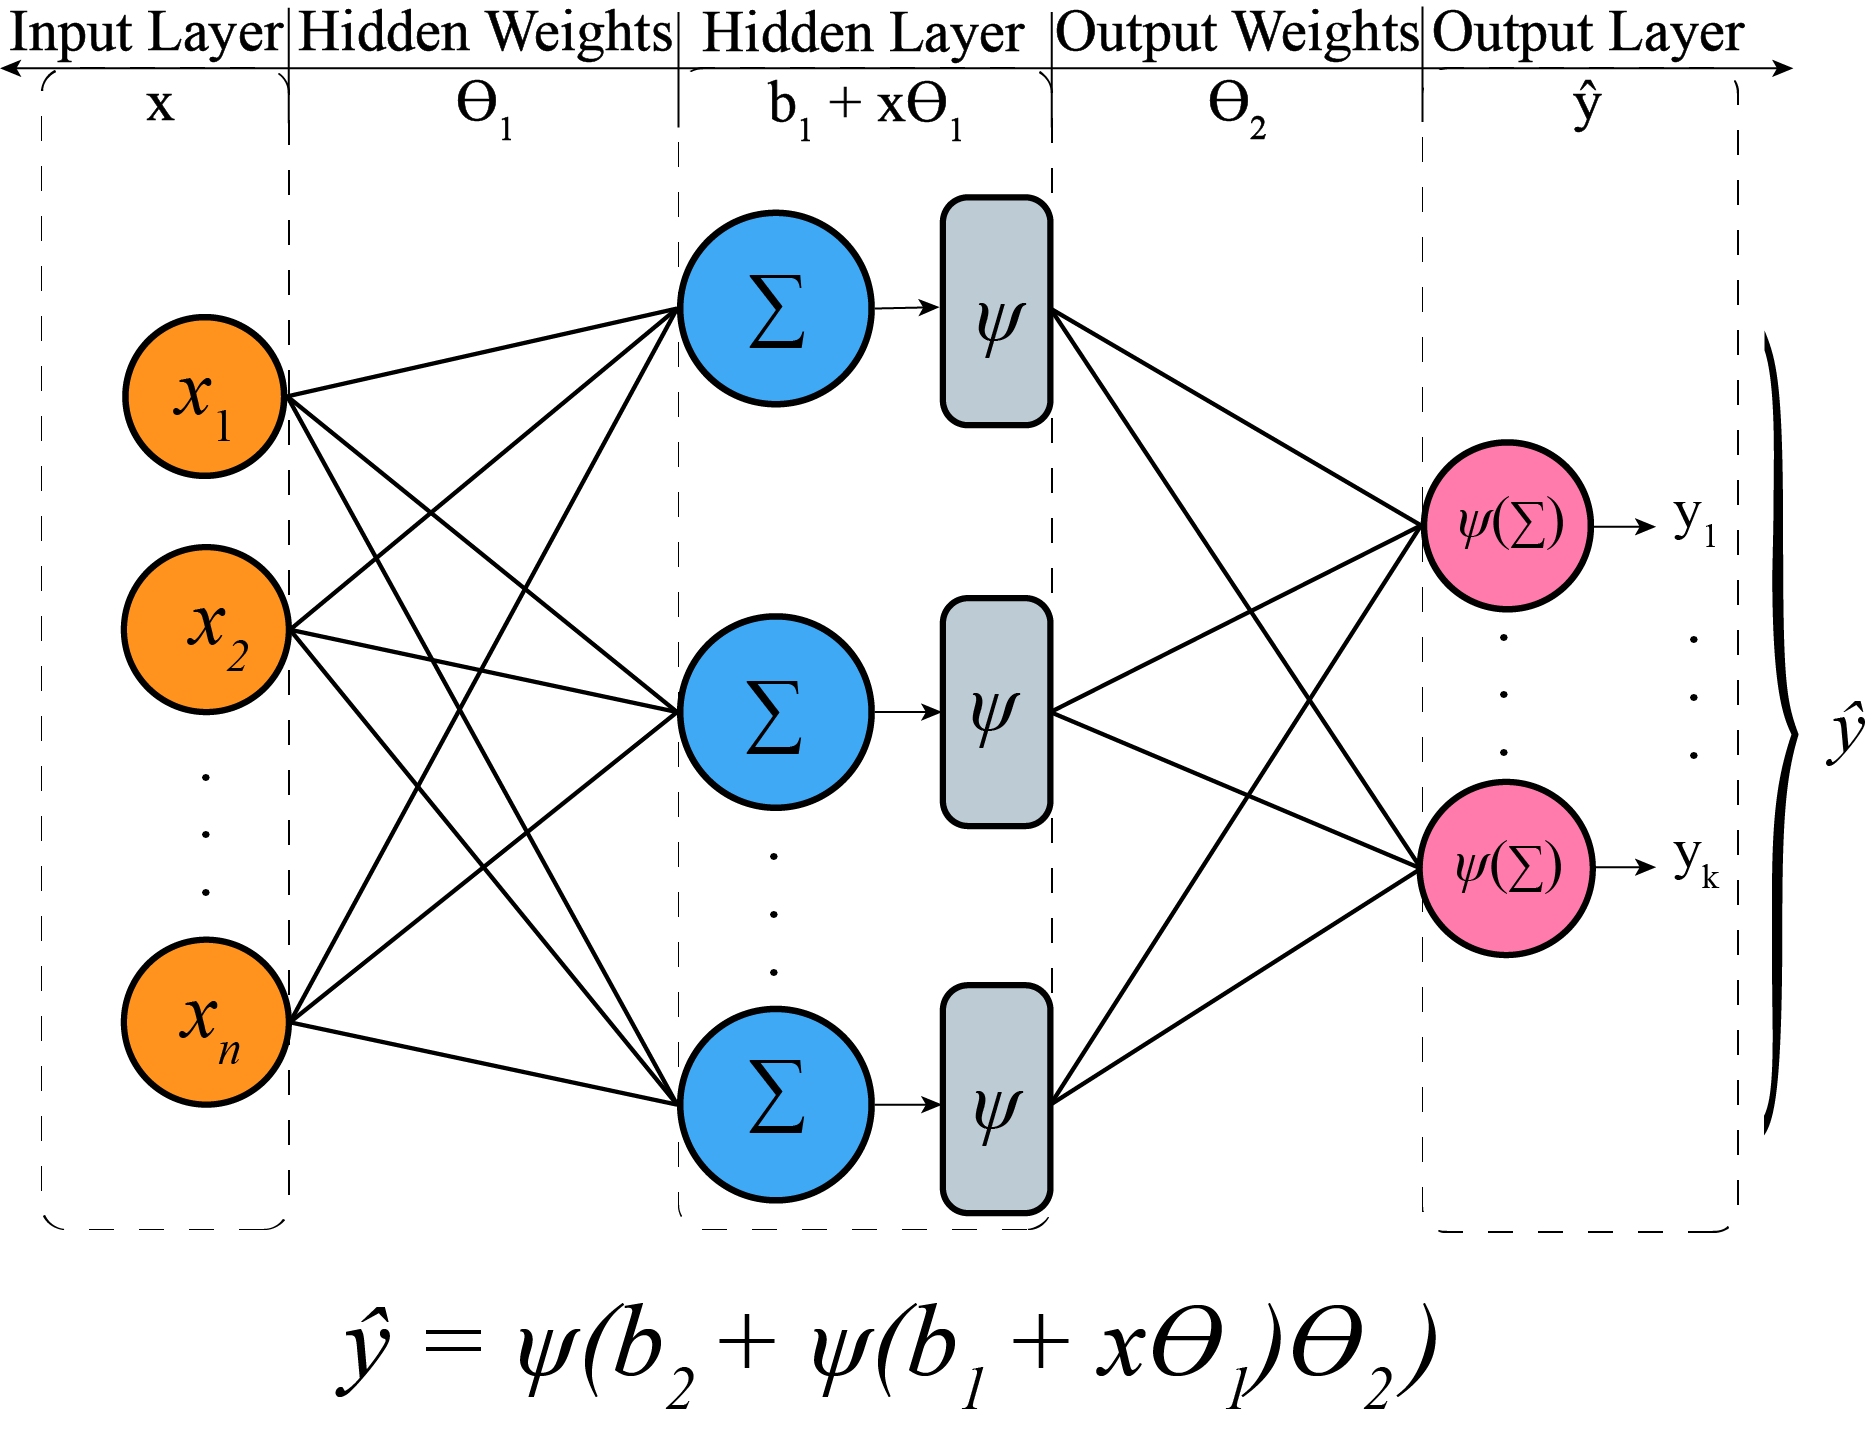
\includegraphics[width=.55\linewidth, height = 5cm]{img/mlp.png}\label{fig:nonlinearsep}\hfill
        	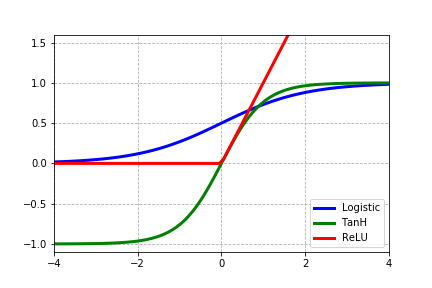
\includegraphics[width=.4\linewidth, height = 5cm]{img/actfunc.png}\label{fig:linearsep}
        \end{subfigure}
        
        \caption{The original data (left) is not linearly separable, that is, there does not exists a hyperplane capable of
            separating the red curve from the blue curve. The transformation $h = \sigma(Wx + b)$ project the input x into a new space
        (right) where it's easy to find a separating hyperplane. Images taken from: \url{http://colah.github.io/posts/2014-03-NN-Manifolds-Topology/}}\label{fig:linear-layer-viz}
	\end{figure}
	
	\begin{figure}
    \centering
    \begin{subfigure}[b]{0.55\textwidth}
        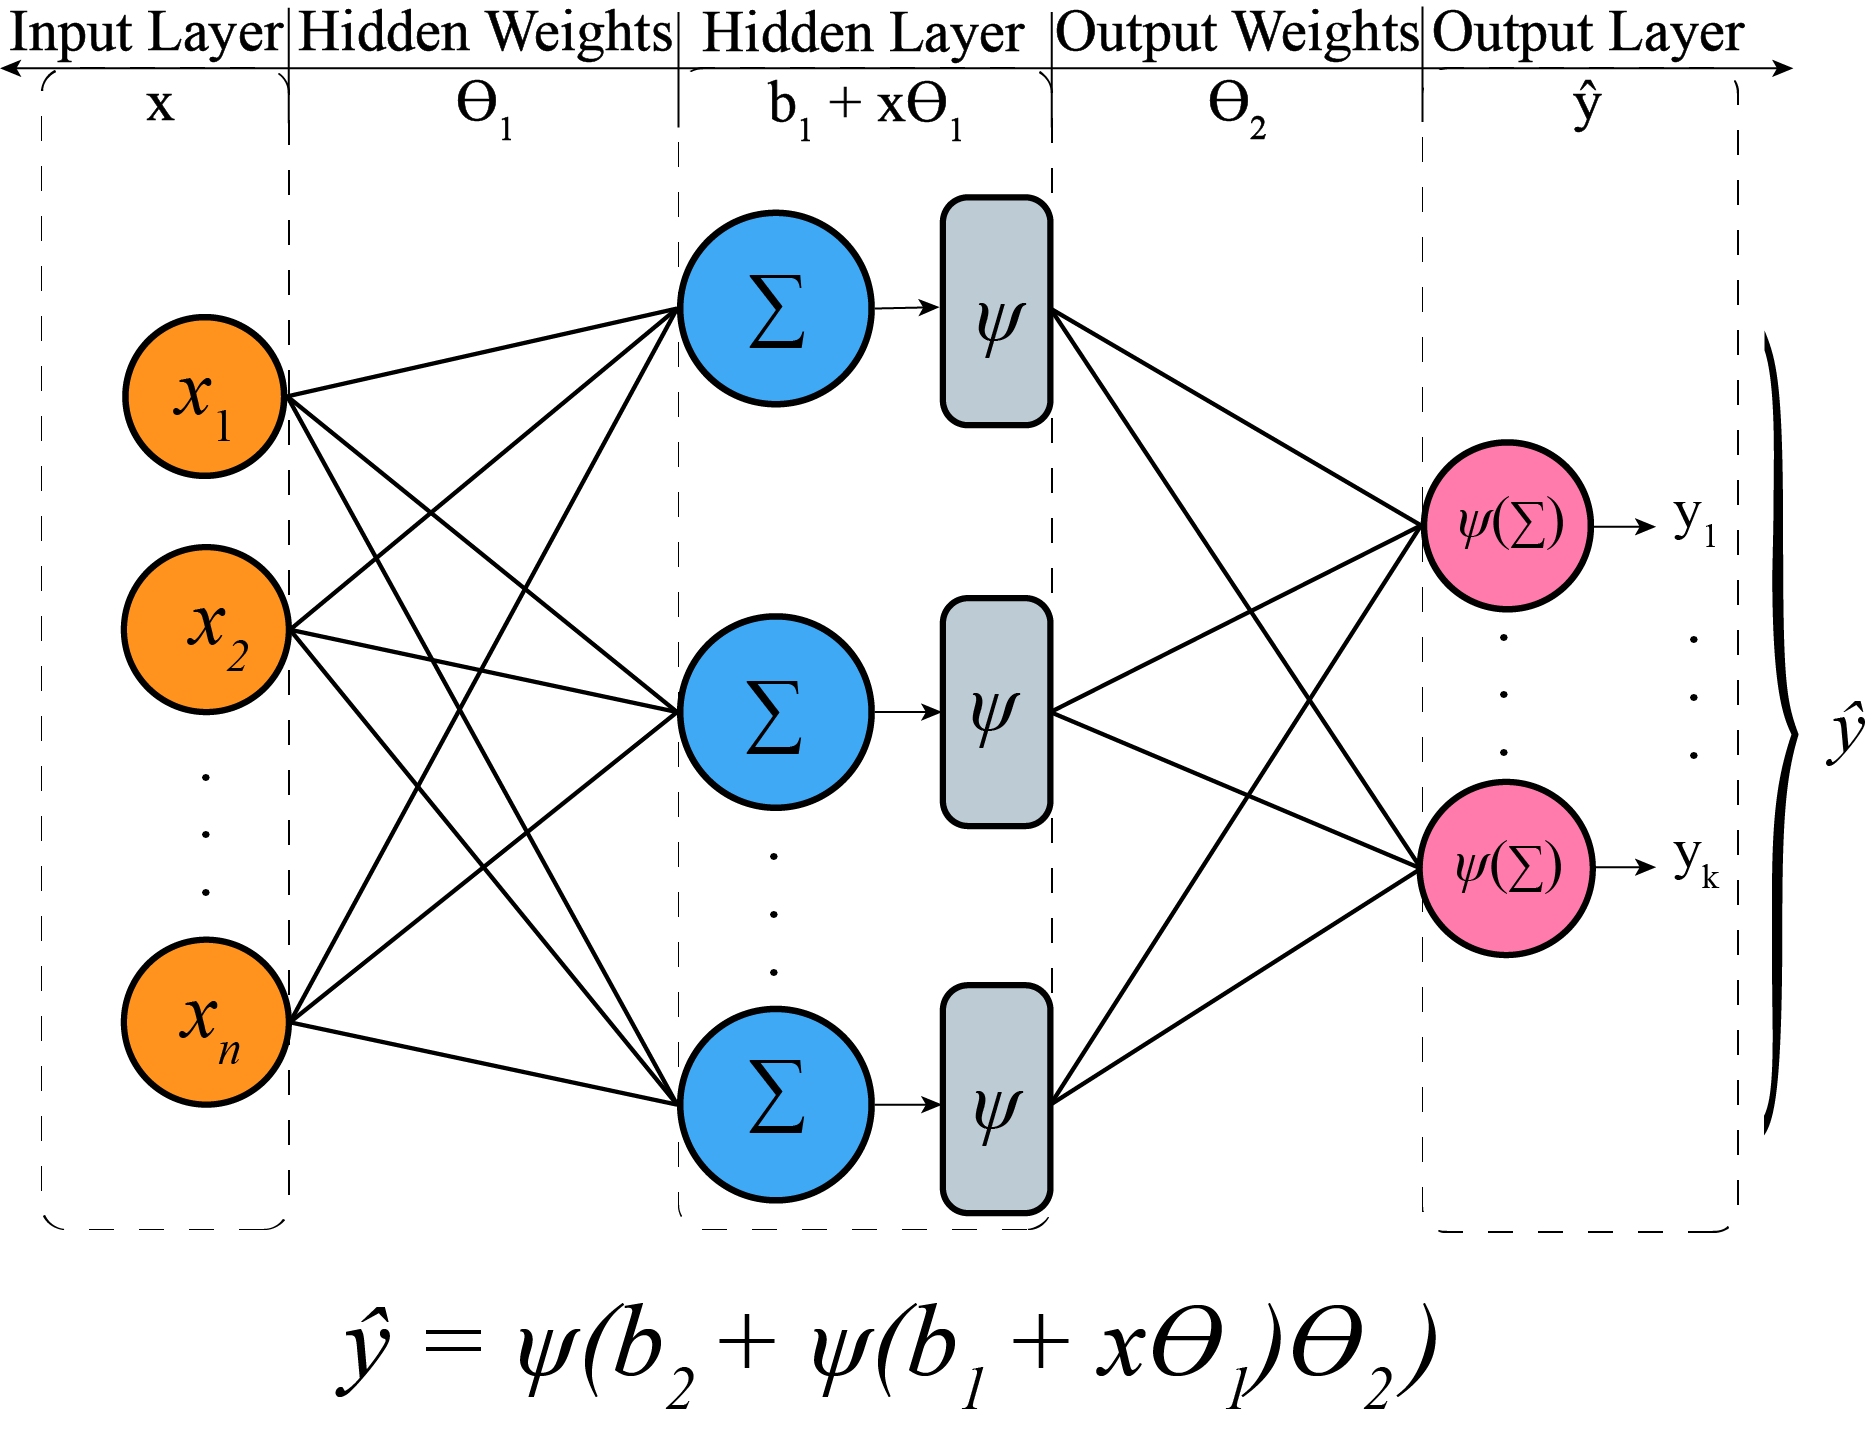
\includegraphics[height = 6cm, width=\textwidth]{img/mlp.png}
        \caption{Feed Forward Multilayer Perceptron}
        \label{fig:mlp}
    \end{subfigure}
    \hfill
    \begin{subfigure}[b]{0.44\textwidth}
        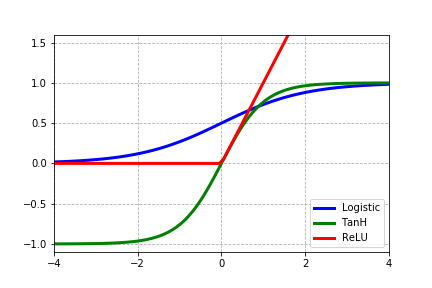
\includegraphics[height = 6.5cm, width=\textwidth]{img/actfunc.png}
        \caption{Common Activation Functions, $\psi$}
        \label{fig:tiger}
    \end{subfigure}
    \caption{Pictures of animals}\label{fig:animals}
\end{figure}